\section{Development of Methods}

\hspace*{0.3cm} All of the methods outlined in preceding chapters were developed in \textit{RStudio} and are stored in a public code repository on \textit{GitHub}. Initial development and testing of all the packages and libraries was completed using \textit{R Markdown} notebooks, which allow for coding in chunks with explanation in markdown text. These netbooks are kept in the code repo to serve as more explanatory documents demonstrating how all the scripts and datasets work in conjunction with one another. \\
The resulting and final scripts are kept in the code repository as well. The final scripts were developed to use the output from one another and to produce intermediate outputs so that small studies could be conducted. How the scripts work with one another is mapped out in the "Script Map" in Figure 3.1.\\

\begin{figure}
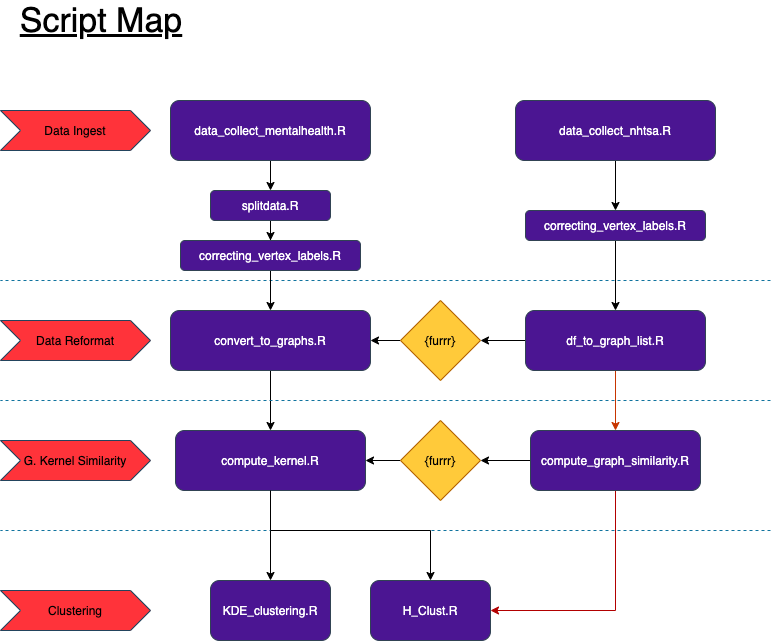
\includegraphics[width=6in]{Content/Images/ScriptMap.png}\\
\caption{Development script map that describes how all modules work together from data ingest to final analysis.}
\end{figure} 

 The Script Map shows how these R scripts can be used for either standard computation, in the case of the NHTSA dataset, or parallel computation, as was used in the reddit dataset. Parallel computation was completed through use of the \texttt{\{furrr\}}, an R package that makes parallization of functions similar to mapping functions from the popular \texttt{\{purrr\}} package. The \texttt{\{furrr\}} package works by splitting the computation among ``workers", or cores, in the CPU. This takes full advantage of the processing capabilities of the machine; instead of letting 1 core do all of the work, we can use many more. Implementation of a parallel option was necessary because computational time for a list of graph objects grows rapidly as the number of graphs in the list increases. A small study was conducted on the reddit dataset to plot this relationship.\\
 
\begin{figure}
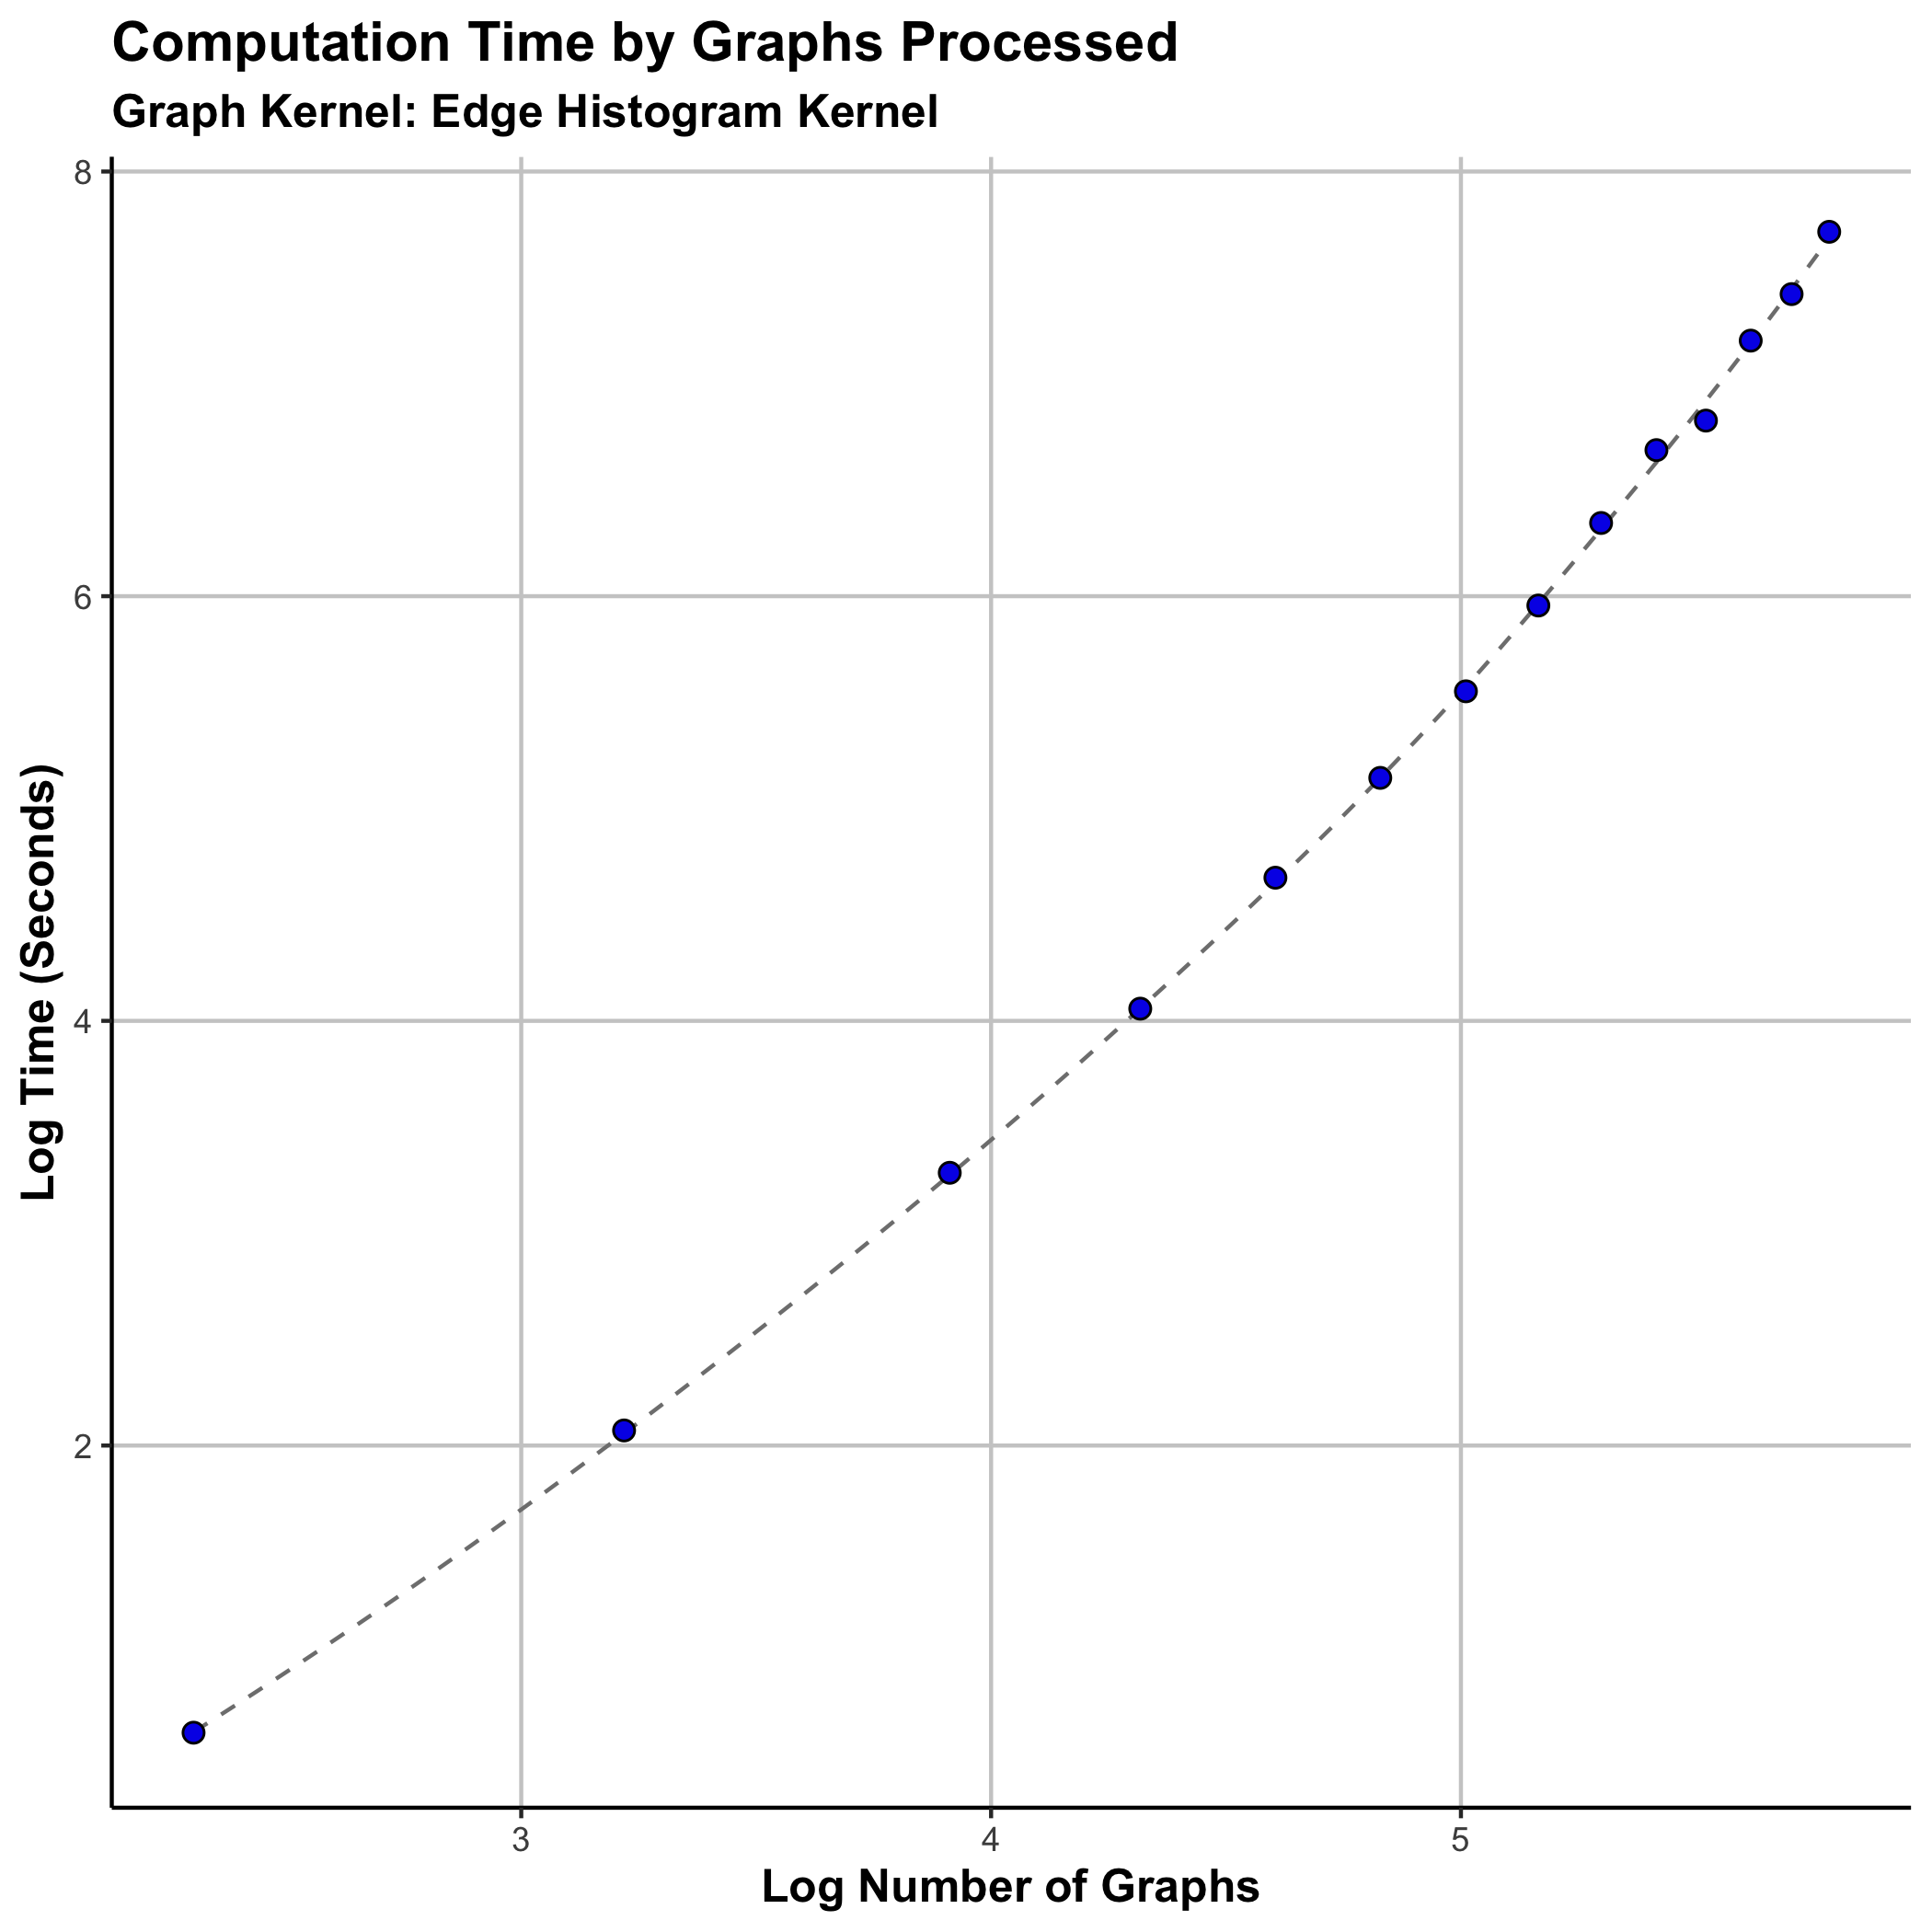
\includegraphics[width=6in]{Content/Images/edgeHistTimePlot.png}\\
\caption{Small study on computation time as a function of the number of graphs in list to be processed. Data from reddit used.}
\end{figure}
 
Above, in Figure 3.2, there is strong evidence that the computation time follows $O(n^2)$. For this reason, the parallel workflow was developed\textemdash to handle datasets with a large number of documents to compare. Even though the amount of text per document in the NHTSA dataset is much larger than the amount of text per document in the reddit dataset, the reddit dataset takes much longer to compute. \\

Referring back to the Script Map, either workflow is decomposed into four steps: Data Ingest, Data Reform, Graph Kernel Similarity, and Clustering. This is the basic work flow developed here. There are some things to note in the Script Map.\\ 

First, vertex labels need corrected to work with the \texttt{\{graphkernels\}} package. This is done through reassignment of all text vertex labels to be a scalar value. The labels are mapped from the union of two graphs' labels to values ranging from $1-n$, where $n$ is the size of the text label set from the union. This script is run within the \texttt{convert\char`_to\char`_graphs.R} script, so it operates on two graphs at a time as it iterates through the whole graph set of concern.\\

Second, the scripts routed through \texttt{\{furrr\}} are functions which are parallelized in the \texttt{convert\char`_to\char`_graphs.R} and \texttt{compute\char`_kernel.R} scripts. These parallelized scripts are done so through a function being executed with no argument, so the dataset which they consider is hard coded into the script. This is not good from a reproducibility aspect, but it is well documented in the code and in the repository, and has reproducible results. \\

Third, the \texttt{splitdata.R} function is there to simply split up the dataset from reddit, which would be too large to store in the repository on GitHub. This segmentation of the data still allows for workflow and reproducibility, since the datasets can all be read in to the environment all the same. \\

Lastly, a KDE clustering analysis was not performed on the NHTSA dataset, as that dataset has few observations ($N=48$) and will not perform well with the density estimation methods developed here; there would be too few observations to generate a number of local maxima/minima needed to apply the clustering methods developed. \\

 